\documentclass{standalone}
\usepackage{tikz}
\usetikzlibrary{patterns, positioning}

\begin{document}
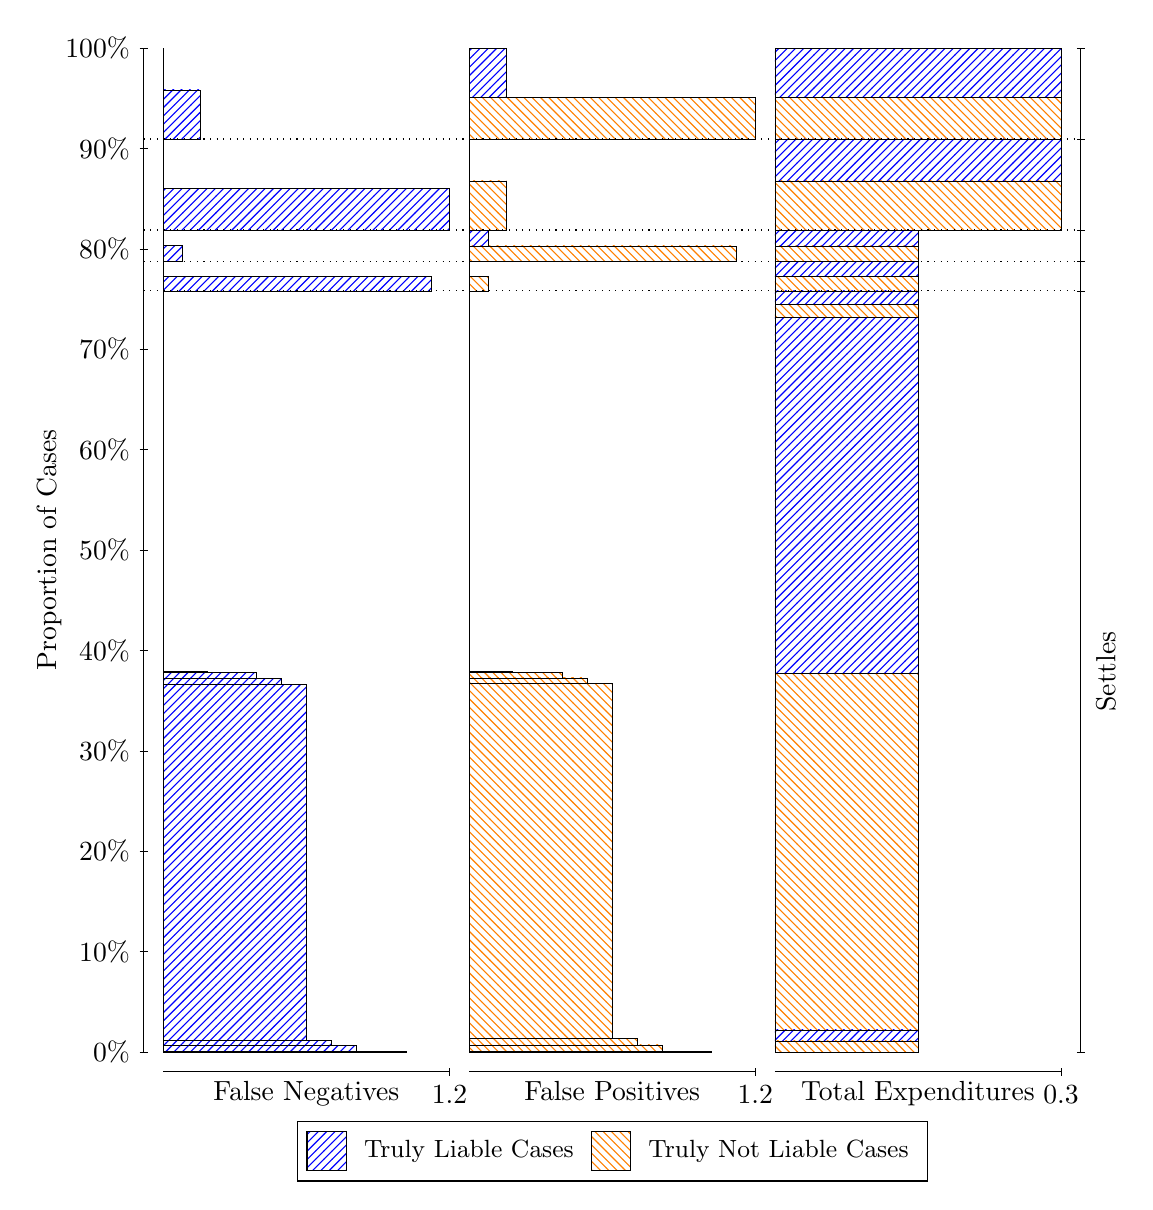
\begin{tikzpicture}
\draw[black, very thin] (1.5,1.75) -- (1.5,14.5);
\node[rotate=90, anchor=center] at (0.3, 8.125) {Proportion of Cases};
\draw[black, very thin] (1.45,1.75) -- (1.55,1.75);
\node[anchor=east] at (1.45, 1.75) {0\%};
\draw[black, very thin] (1.45,3.025) -- (1.55,3.025);
\node[anchor=east] at (1.45, 3.025) {10\%};
\draw[black, very thin] (1.45,4.3) -- (1.55,4.3);
\node[anchor=east] at (1.45, 4.3) {20\%};
\draw[black, very thin] (1.45,5.575) -- (1.55,5.575);
\node[anchor=east] at (1.45, 5.575) {30\%};
\draw[black, very thin] (1.45,6.85) -- (1.55,6.85);
\node[anchor=east] at (1.45, 6.85) {40\%};
\draw[black, very thin] (1.45,8.125) -- (1.55,8.125);
\node[anchor=east] at (1.45, 8.125) {50\%};
\draw[black, very thin] (1.45,9.4) -- (1.55,9.4);
\node[anchor=east] at (1.45, 9.4) {60\%};
\draw[black, very thin] (1.45,10.675) -- (1.55,10.675);
\node[anchor=east] at (1.45, 10.675) {70\%};
\draw[black, very thin] (1.45,11.95) -- (1.55,11.95);
\node[anchor=east] at (1.45, 11.95) {80\%};
\draw[black, very thin] (1.45,13.225) -- (1.55,13.225);
\node[anchor=east] at (1.45, 13.225) {90\%};
\draw[black, very thin] (1.45,14.5) -- (1.55,14.5);
\node[anchor=east] at (1.45, 14.5) {100\%};

\draw[black, very thin] (13.4,1.75) -- (13.4,14.5);
\draw[black, very thin] (13.35,1.75) -- (13.45,1.75);
\node[anchor=west] at (13.35, 1.75) {};
\draw[black, very thin] (13.35,11.415) -- (13.45,11.415);
\node[anchor=west] at (13.35, 11.415) {};
\draw[black, very thin] (13.35,11.788) -- (13.45,11.788);
\node[anchor=west] at (13.35, 11.788) {};
\draw[black, very thin] (13.35,12.189) -- (13.45,12.189);
\node[anchor=west] at (13.35, 12.189) {};
\draw[black, very thin] (13.35,13.345) -- (13.45,13.345);
\node[anchor=west] at (13.35, 13.345) {};
\draw[black, very thin] (13.35,14.5) -- (13.45,14.5);
\node[anchor=west] at (13.35, 14.5) {};

\draw[black, very thin, pattern color=blue, pattern=north east lines] (1.75,1.75) rectangle (4.8304,1.76);
\draw[black, very thin, pattern color=blue, pattern=north east lines] (1.75,1.76) rectangle (4.5145,1.7612);
\draw[black, very thin, pattern color=blue, pattern=north east lines] (1.75,1.7612) rectangle (4.1986,1.8303);
\draw[black, very thin, pattern color=blue, pattern=north east lines] (1.75,1.8303) rectangle (3.8826,1.8997);
\draw[black, very thin, pattern color=blue, pattern=north east lines] (1.75,1.8997) rectangle (3.5667,6.4142);
\draw[black, very thin, pattern color=blue, pattern=north east lines] (1.75,6.4142) rectangle (3.2507,6.4917);
\draw[black, very thin, pattern color=blue, pattern=north east lines] (1.75,6.4917) rectangle (2.9348,6.5715);
\draw[black, very thin, pattern color=blue, pattern=north east lines] (1.75,6.5715) rectangle (2.6188,6.5753);
\draw[black, very thin, pattern color=blue, pattern=north east lines] (1.75,6.5753) rectangle (2.3029,6.5828);
\draw[black, very thin, pattern color=orange, pattern=north west lines] (1.75,6.5828) rectangle (1.75,11.415);
\draw[black, very thin, pattern color=blue, pattern=north east lines] (1.75,11.415) rectangle (5.1464,11.601);
\draw[black, very thin, pattern color=orange, pattern=north west lines] (1.75,11.601) rectangle (1.75,11.788);
\draw[black, very thin, pattern color=blue, pattern=north east lines] (1.75,11.788) rectangle (1.987,11.99);
\draw[black, very thin, pattern color=orange, pattern=north west lines] (1.75,11.99) rectangle (1.75,12.189);
\draw[black, very thin, pattern color=blue, pattern=north east lines] (1.75,12.189) rectangle (5.3833,12.72);
\draw[black, very thin, pattern color=orange, pattern=north west lines] (1.75,12.72) rectangle (1.75,13.345);
\draw[black, very thin, pattern color=blue, pattern=north east lines] (1.75,13.345) rectangle (2.2239,13.969);
\draw[black, very thin, pattern color=orange, pattern=north west lines] (1.75,13.969) rectangle (1.75,14.5);
\draw[black, very thin, pattern color=orange, pattern=north west lines] (5.6333,1.75) rectangle (8.7138,1.7573);
\draw[black, very thin, pattern color=orange, pattern=north west lines] (5.6333,1.7573) rectangle (8.3978,1.7613);
\draw[black, very thin, pattern color=orange, pattern=north west lines] (5.6333,1.7613) rectangle (8.0819,1.8409);
\draw[black, very thin, pattern color=orange, pattern=north west lines] (5.6333,1.8409) rectangle (7.7659,1.9181);
\draw[black, very thin, pattern color=orange, pattern=north west lines] (5.6333,1.9181) rectangle (7.45,6.4319);
\draw[black, very thin, pattern color=orange, pattern=north west lines] (5.6333,6.4319) rectangle (7.1341,6.5006);
\draw[black, very thin, pattern color=orange, pattern=north west lines] (5.6333,6.5006) rectangle (7.1341,6.5018);
\draw[black, very thin, pattern color=orange, pattern=north west lines] (5.6333,6.5018) rectangle (6.8181,6.5713);
\draw[black, very thin, pattern color=orange, pattern=north west lines] (5.6333,6.5713) rectangle (6.5022,6.5725);
\draw[black, very thin, pattern color=orange, pattern=north west lines] (5.6333,6.5725) rectangle (6.1862,6.5826);
\draw[black, very thin, pattern color=blue, pattern=north east lines] (5.6333,6.5826) rectangle (5.6333,11.415);
\draw[black, very thin, pattern color=orange, pattern=north west lines] (5.6333,11.415) rectangle (5.8703,11.602);
\draw[black, very thin, pattern color=blue, pattern=north east lines] (5.6333,11.602) rectangle (5.6333,11.788);
\draw[black, very thin, pattern color=orange, pattern=north west lines] (5.6333,11.788) rectangle (9.0297,11.988);
\draw[black, very thin, pattern color=blue, pattern=north east lines] (5.6333,11.988) rectangle (5.8703,12.189);
\draw[black, very thin, pattern color=orange, pattern=north west lines] (5.6333,12.189) rectangle (6.1072,12.814);
\draw[black, very thin, pattern color=blue, pattern=north east lines] (5.6333,12.814) rectangle (5.6333,13.345);
\draw[black, very thin, pattern color=orange, pattern=north west lines] (5.6333,13.345) rectangle (9.2667,13.875);
\draw[black, very thin, pattern color=blue, pattern=north east lines] (5.6333,13.875) rectangle (6.1072,14.5);
\draw[black, very thin, pattern color=orange, pattern=north west lines] (9.5167,1.75) rectangle (11.333,1.8905);
\draw[black, very thin, pattern color=blue, pattern=north east lines] (9.5167,1.8905) rectangle (11.333,2.0302);
\draw[black, very thin, pattern color=orange, pattern=north west lines] (9.5167,2.0302) rectangle (11.333,6.5541);
\draw[black, very thin, pattern color=blue, pattern=north east lines] (9.5167,6.5541) rectangle (11.333,11.079);
\draw[black, very thin, pattern color=orange, pattern=north west lines] (9.5167,11.079) rectangle (11.333,11.247);
\draw[black, very thin, pattern color=blue, pattern=north east lines] (9.5167,11.247) rectangle (11.333,11.415);
\draw[black, very thin, pattern color=orange, pattern=north west lines] (9.5167,11.415) rectangle (11.333,11.602);
\draw[black, very thin, pattern color=blue, pattern=north east lines] (9.5167,11.602) rectangle (11.333,11.788);
\draw[black, very thin, pattern color=orange, pattern=north west lines] (9.5167,11.788) rectangle (11.333,11.988);
\draw[black, very thin, pattern color=blue, pattern=north east lines] (9.5167,11.988) rectangle (11.333,12.189);
\draw[black, very thin, pattern color=orange, pattern=north west lines] (9.5167,12.189) rectangle (13.15,12.814);
\draw[black, very thin, pattern color=blue, pattern=north east lines] (9.5167,12.814) rectangle (13.15,13.345);
\draw[black, very thin, pattern color=orange, pattern=north west lines] (9.5167,13.345) rectangle (13.15,13.875);
\draw[black, very thin, pattern color=blue, pattern=north east lines] (9.5167,13.875) rectangle (13.15,14.5);
\draw[black, dotted] (1.5,11.415) -- (13.4,11.415);
\draw[black, dotted] (1.5,11.788) -- (13.4,11.788);
\draw[black, dotted] (1.5,12.189) -- (13.4,12.189);
\draw[black, dotted] (1.5,13.345) -- (13.4,13.345);
\draw[black, very thin] (1.75,1.5) -- (5.3833,1.5);
\node[anchor=north] at (3.5667, 1.5) {False Negatives};
\draw[black, very thin] (5.3833,1.45) -- (5.3833,1.55);
\node[anchor=north] at (5.3833, 1.45) {1.2};

\draw[black, very thin] (5.6333,1.5) -- (9.2667,1.5);
\node[anchor=north] at (7.45, 1.5) {False Positives};
\draw[black, very thin] (9.2667,1.45) -- (9.2667,1.55);
\node[anchor=north] at (9.2667, 1.45) {1.2};

\draw[black, very thin] (9.5167,1.5) -- (13.15,1.5);
\node[anchor=north] at (11.333, 1.5) {Total Expenditures};
\draw[black, very thin] (13.15,1.45) -- (13.15,1.55);
\node[anchor=north] at (13.15, 1.45) {0.3};

\node[black, centered, rotate=90] at (13.72, 6.5827) {Settles};





\draw (7.449999999999999,1.5) node[draw=none] (baseCoordinate) {};
\begin{scope}[align=center]
        \matrix[scale=0.5, draw=black, below=0.5cm of baseCoordinate, nodes={draw}, column sep=0.1cm]{
            \node[rectangle, draw, minimum width=0.5cm, minimum height=0.5cm, pattern=north east lines, pattern color=blue] {}; &
            \node[draw=none, font=\small] (B) {Truly Liable Cases}; &
            \node[rectangle, draw, minimum width=0.5cm, minimum height=0.5cm, pattern=north west lines, pattern color=orange] {}; &
            \node[draw=none, font=\small] (B) {Truly Not Liable Cases}; \\
            };
\end{scope}

\end{tikzpicture}
\end{document}